\begin{frame}
	\frametitle{ Problems with MH}
	\begin{itemize}
		\item[] To assert proposal's adequacy
		\begin{itemize}
			\item[]	generate $ U \sim \mathfrak{U}(0,1) $
			\item[] accept $y$ if $U \leq \frac{h(y)q(y,x)}{h(x)q(x,y)} \wedge 1$ 
			\item[] if $q(x,y) = q(y,x)$  
				$$U \leq \frac{h(y)}{h(x)} \wedge 1$$
		\end{itemize}

		\item[] Problem: if $\pi$ is multimodial we get stuck in certain region of the state-space
	\end{itemize}
\end{frame}

	%%%%%%%%%%%%%%%%%%%%%%%%%%%%%%%%%%%%%%%%%%%%%%%%%%%%%%%%%%%%%%

\begin{frame}
		\frametitle{Liang and Wong 2001}
	
	\begin{itemize}
		\item[] $$ f(x) = 
			\sum_{i=1}^{20} \frac{\omega_i}{ \sigma_i \sqrt{2 \pi} } \exp \Big( -\frac{(x - \mu_i)'(x - \mu_i)}{2 \sigma_i^2} \Big) $$

		\item[]
		\item[] where $\sigma_1 = \dots = \sigma_{20} = 0.1$, $\omega_1 = \dots = \omega_{20} = 0.05 $
		\item[] and the means $\mu_i$ are given by

		\item[] 
\begin{table}[ht]
\centering
\begin{tabular}{rrrrrrrrrr}
  \hline
1 & 2 & 3 & 4 & 5 & 6 & 7 & 8 & 9 & 10 \\ 
  \hline
2.18 & 8.67 & 4.24 & 8.41 & 3.93 & 3.25 & 1.70 & 4.59 & 6.91 & 6.87 \\ 
  5.76 & 9.59 & 8.48 & 1.68 & 8.82 & 3.47 & 0.50 & 5.60 & 5.81 & 5.40 \\ 
   \hline
\end{tabular}
\end{table}

		\item[]
\begin{table}[ht]
\centering
\begin{tabular}{rrrrrrrrrr}
  \hline
11 & 12 & 13 & 14 & 15 & 16 & 17 & 18 & 19 & 20 \\ 
  \hline
5.41 & 2.70 & 4.98 & 1.14 & 8.33 & 4.93 & 1.83 & 2.26 & 5.54 & 1.69 \\ 
  2.65 & 7.88 & 3.70 & 2.39 & 9.50 & 1.50 & 0.09 & 0.31 & 6.86 & 8.11 \\ 
   \hline
\end{tabular}
\end{table}
	\end{itemize} 	

			
\end{frame}

	%%%%%%%%%%%%%%%%%%%%%%%%%%%%%%%%%%%%%%%%%%%%%%%%%%%%%%%%%%%%%%


\begin{frame}
		\frametitle{toy-example visualised}
	
	\begin{center}
		\begin{figure}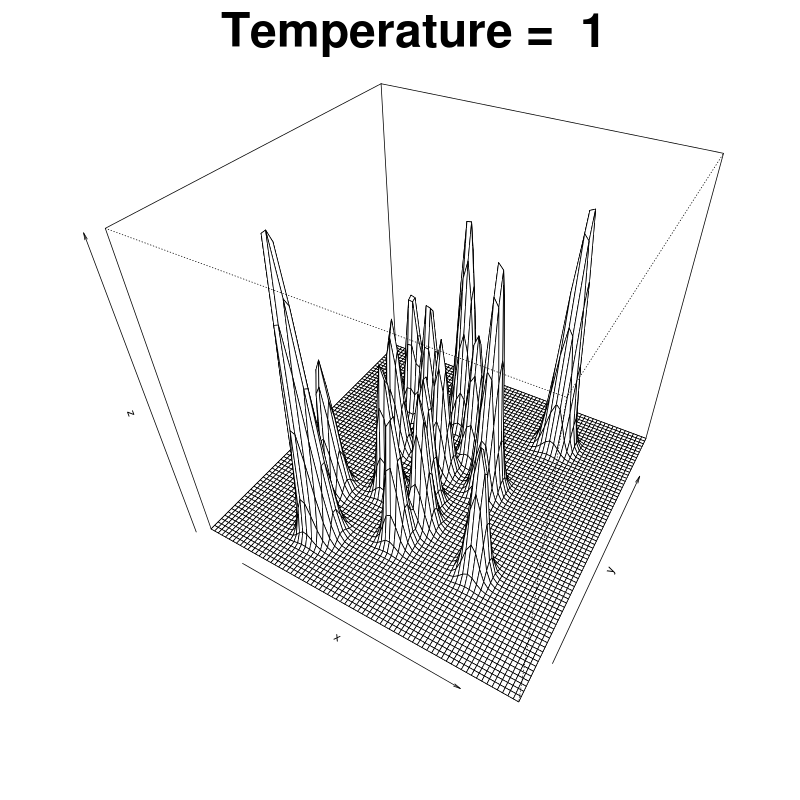
\includegraphics[scale=.3]{./picts/Liang_perspective.png}\end{figure}	
	\end{center}	
		
\end{frame}

\begin{frame}
		\frametitle{toy-example visualised as a contour plot}
	
	\begin{center}
		\begin{figure}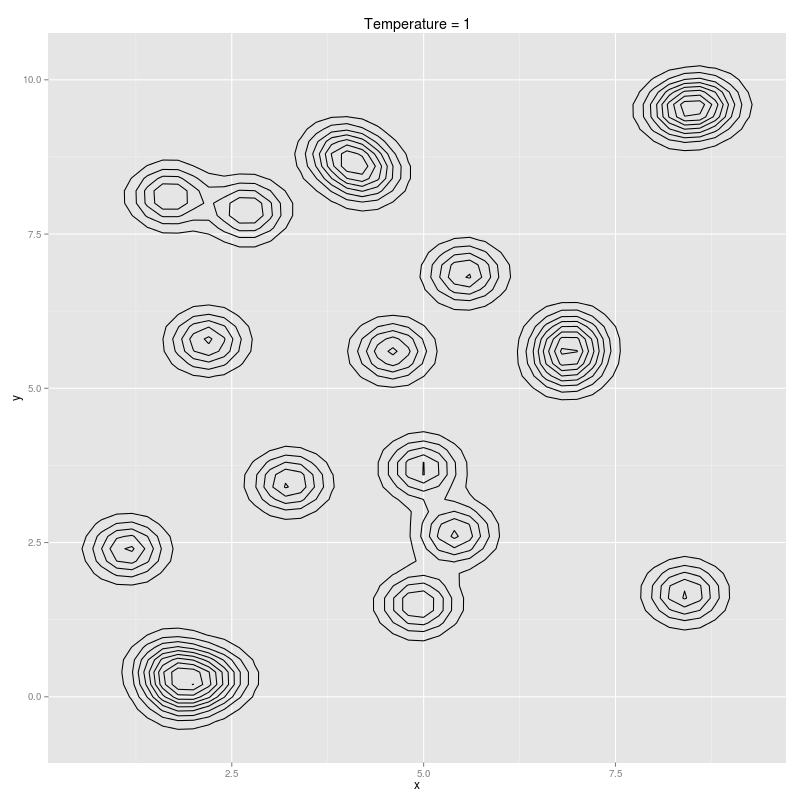
\includegraphics[scale=.25]{./picts/Liang_Contour_plot.png}\end{figure}	
	\end{center}	
		
\end{frame}

	%%%%%%%%%%%%%%%%%%%%%%%%%%%%%%%%%%%%%%%%%%%%%%%%%%%%%%%%%%%%%%

\begin{frame}[plain]

	\begin{center}
		\begin{figure}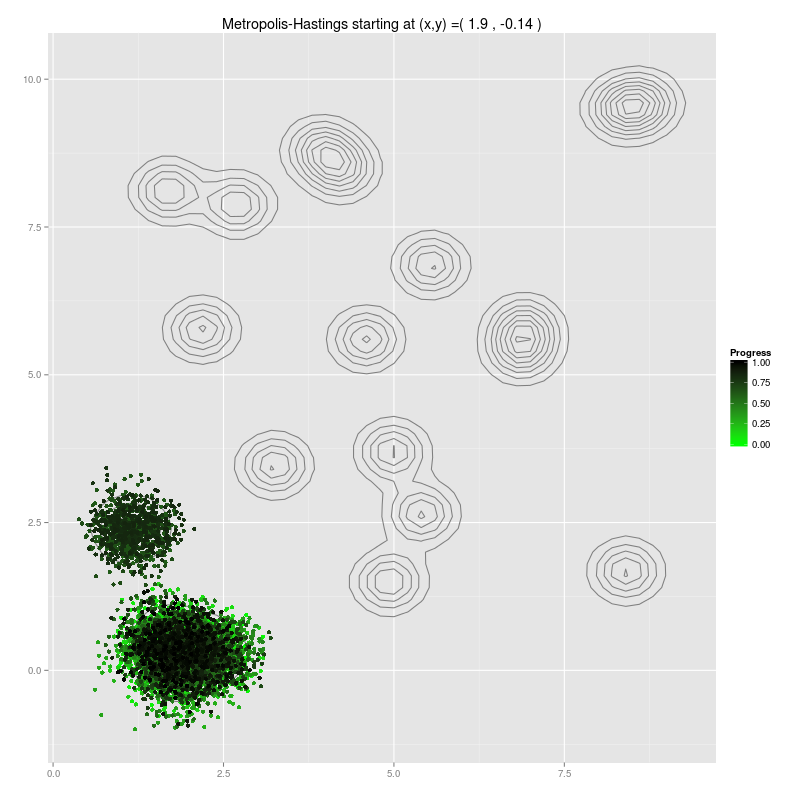
\includegraphics[scale=.31]{./picts/MH_simululation_10000_steps.png}\end{figure}	
	\end{center}	
		
\end{frame}

\begin{frame}[plain]

	\begin{center}
		\begin{figure}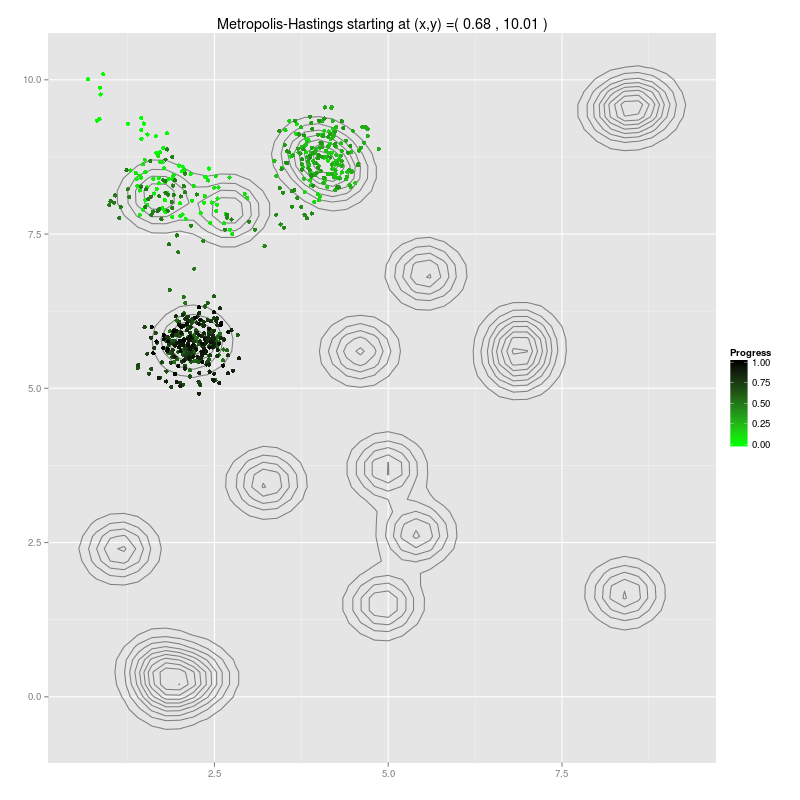
\includegraphics[scale=.31]{./picts/MH_simululation_1000_steps_ex1.png}\end{figure}	
	\end{center}	
		
\end{frame}

\begin{frame}[plain]

	\begin{center}
		\begin{figure}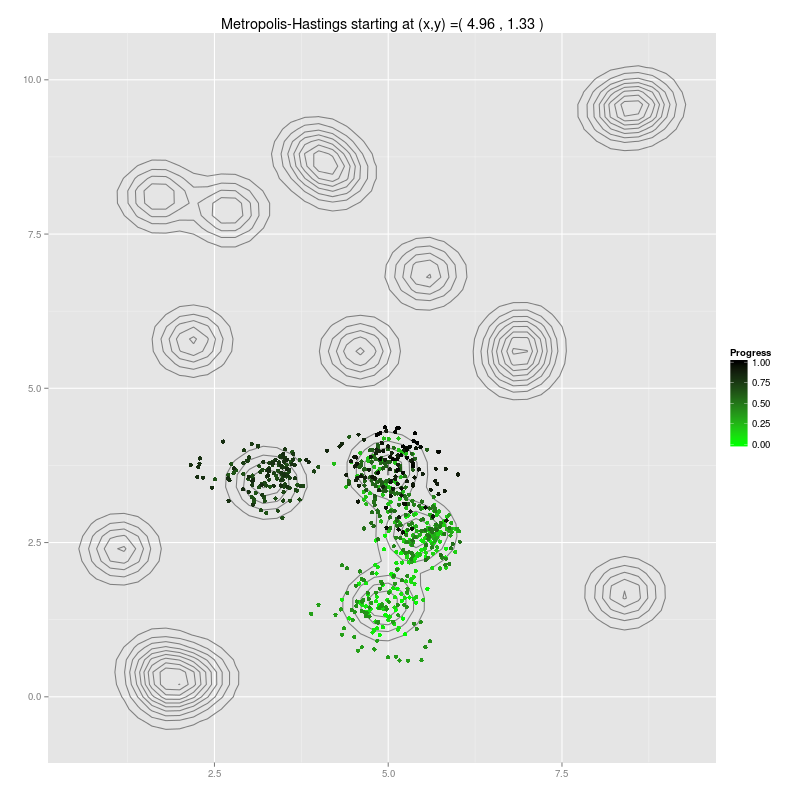
\includegraphics[scale=.31]{./picts/MH_simululation_1000_steps_ex2.png}\end{figure}	
	\end{center}	
		
\end{frame}

	%%%%%%%%%%%%%%%%%%%%%%%%%%%%%%%%%%%%%%%%%%%%%%%%%%%%%%%%%%%%%%


\begin{frame}
	\frametitle{Parallel Tempering in action.}
	\begin{center}
		\begin{figure}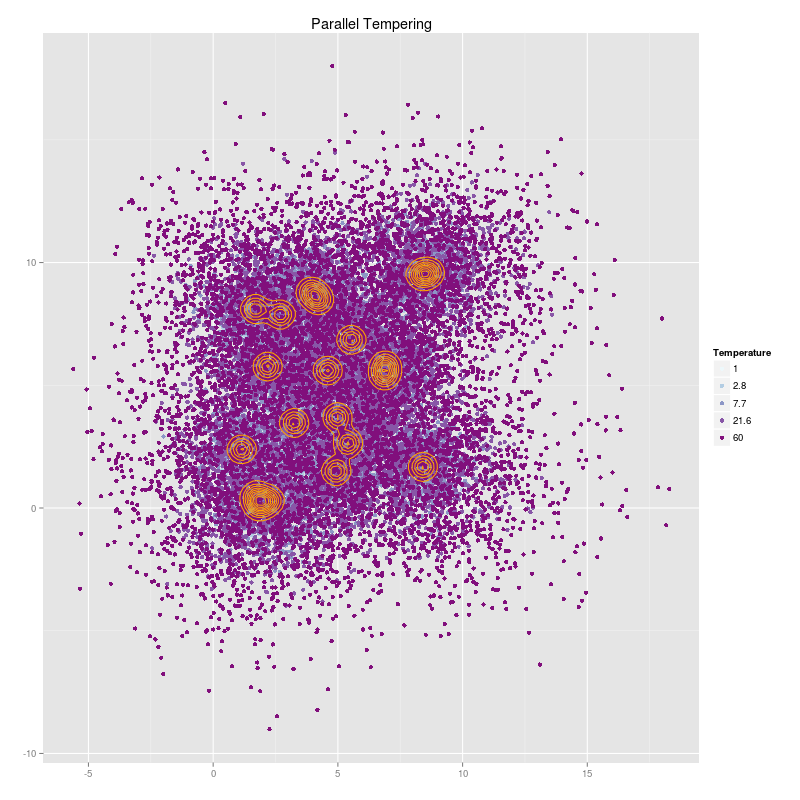
\includegraphics[scale=.28]{./picts/PT_simululation_10000_steps_1.png}\end{figure}	
	\end{center}	
		
\end{frame}

